\chapter{Incoherency} \label{chap:Incoherency}

In this chapter the blending operator is analyzed in greater detail. Then a measure for incoherency will be introduced and the role of incoherency for deblending will be discussed.

\section{Analysis of the Blending Matrix} \label{sec:BlendingMatrix}

In order to optimize the blended acquisition design, one must understand the properties of the blending matrix $\mathbf{\Gamma}$ and its influence on the deblending performance.

The blending matrix $\mathbf{\Gamma}$ determines the pseudo-deblended data,

\begin{equation}
	\mathbf{P}_{ps} = \mathbf{P \Gamma \Gamma}^H,
	\label{eq:Ch-Theory-Pseudo-Deblended-Data}
\end{equation}

which are a superposition of the unblended data, $\mathbf{P}$, and the blending noise, $\mathbf{N}$,

\begin{equation}
	\mathbf{P}_{ps} = \mathbf{P} + \mathbf{N}.
	\label{eq:Ch-Theory-PseudoSuperposition}
\end{equation}

The more incoherent the blending noise, $\mathbf{N}$, the better it can be removed by noise filters.

In the following the effect of the blending matrix, $\mathbf{\Gamma}$, on the matrix product $\mathbf{\Gamma \Gamma}^H$ and on the pseudo-deblended data is analyzed. For simplicity, it is assumed that all shots are equal in strength and fire the same signature into the earth. This means that the blending matrix, $\mathbf{\Gamma}$, only contains phase shift terms, $\mathrm{e}^{-j \omega \Delta t}$, with an amplitude equal to 1 or 0. It is also assumed that each shot is fired only once, unlike e.g. the shot repetition case \citep{Sixue}.

Each row of $\mathbf{\Gamma}$ represents a shot $k$, and each column of $\mathbf{\Gamma}^H$ represents a shot $l$ with a complex conjugated phase term (see Figure \ref{fig:Ch-Theory-GGH}). Hence, each element $g_{kl}$ of the matrix $\mathbf{\Gamma \Gamma}^H$ is the dot product between the $k^{th}$ shot and the complex conjugate of the $l^{th}$ shot.

\begin{figure}
	\centering
	\includegraphics[width = \textwidth]{Plots/GGH_v2}
	\caption{Illustration of the matrix product, $\mathbf{\Gamma \Gamma}^H$. In this notation $\Delta t_k$ refers to the phase shift of the shot $k$, and $\Delta t_{kl}$ refers to the phase shift between the shots $k$ and $l$, $\Delta t_{kl} = \Delta t_k - \Delta t_l$.}
	\label{fig:Ch-Theory-GGH}
\end{figure}

Consequently, an element $g_{kl}$ of the matrix product $\mathbf{\Gamma \Gamma}^H$ represents the overlap of the shots $k$ and $l$ for all experiments. The main diagonal of $\mathbf{\Gamma \Gamma}^H$ refers to the overlap of each shot with itself, which of course is perfect and therefore equal to 1. The off diagonal elements of $\mathbf{\Gamma \Gamma}^H$ are either 0 if the associated shots do not overlap, or contain a phase shift, $\mathrm{e}^{\, -j \omega \Delta t_{kl}}$.

\subsection*{Temporal incoherency}

In the following the term "sub-diagonal" will be used to refer to an arbitrary diagonal of the matrix $\mathbf{\Gamma \Gamma}^H$. For example, the $d^{th}$ sub-diagonal includes all the matrix elements $g_{ij}$, which fulfill the condition;

\begin{equation}
	j -i = d.
	\label{eq:Ch-Incoherency-Subdiagonal}
\end{equation}

In equation \ref{eq:Ch-Theory-Pseudo-Deblended-Data} the main diagonal elements of $\mathbf{\Gamma \Gamma}^H$ copy the data matrix, $\mathbf{P}$, while the off-diagonal elements create the blending noise, $\mathbf{N}$. In case of a coherent firing time delay the elements along a sub-diagonal $d$ are in phase. This means that the sub-diagonal elements will shift the columns of the data matrix and apply a coherent phase shift to each of them resulting in the pseudo-deblended receiver gather shown in Figure \ref{fig:Ch-Theory-PseudoCRG-CoherentDelay}. Instead if the elements $g_{ij}$ along a sub-diagonal $d$ are out of phase, they will shift the columns of the data matrix and distort the phase of each column (see Figure \ref{fig:Ch-Theory-PseudoCRG-IncoherentDelay}). 

Figure \ref{fig:Ch-Theory-PseudoCRG-FK-CoherentDelay} and \ref{fig:Ch-Theory-PseudoCRG-FK-IncoherentDelay} display the $f$-$k$-spectra of the pseudo-blended data for constant firing time delays and random firing time delays respectively. In the case of constant firing time delays almost all of the energy maps in the signal cone. In the case of random firing time delays a significant part of the energy maps outside of the signal cone. Therefore, the coherency constraint requires random firing time delays. 

In this thesis the random firing time delays are referred to as temporal incoherency.  

\begin{figure}
	\centering
	\begin{subfigure}[b]{0.3\textwidth}
		\centering
		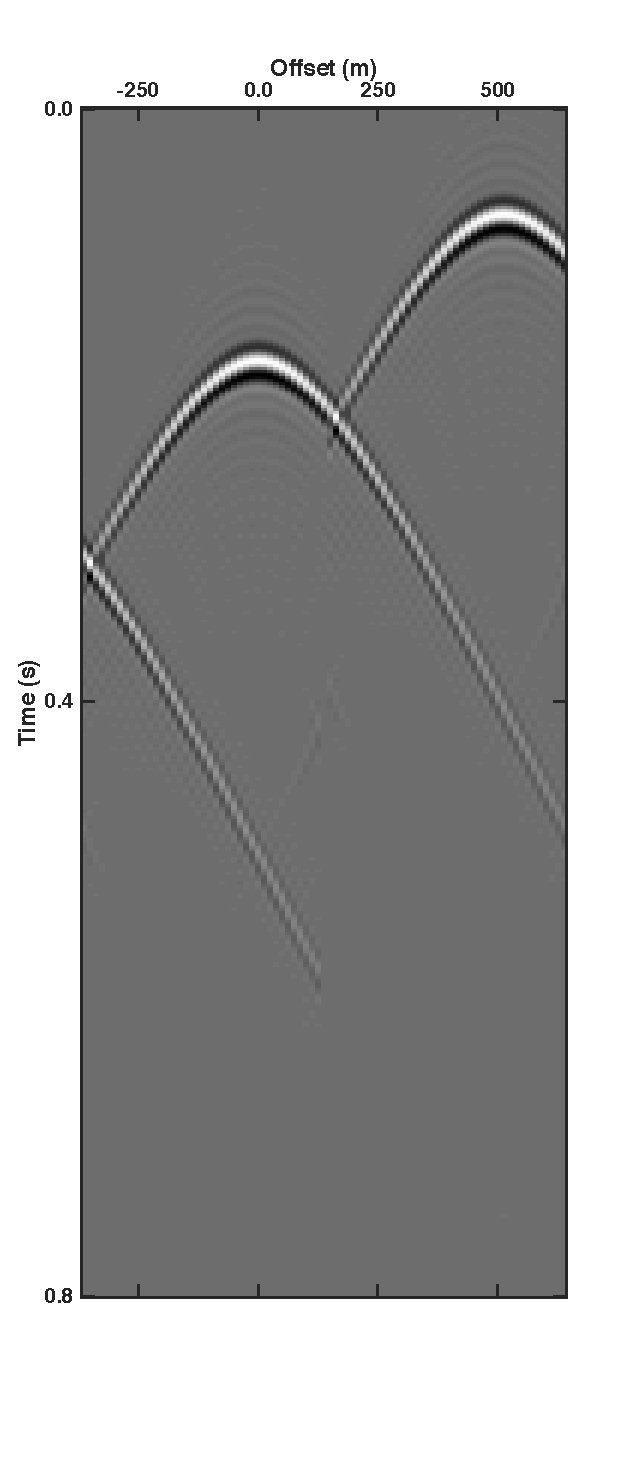
\includegraphics[width = \textwidth]{Plots/Mahdad/25iter/TimeDelay/Pseudo-DeblendedCRG_rec30_coh}
		\caption{}
		\label{fig:Ch-Theory-PseudoCRG-CoherentDelay}
	\end{subfigure}
	%
	\centering
	\begin{subfigure}[b]{0.3\textwidth}
		\centering
		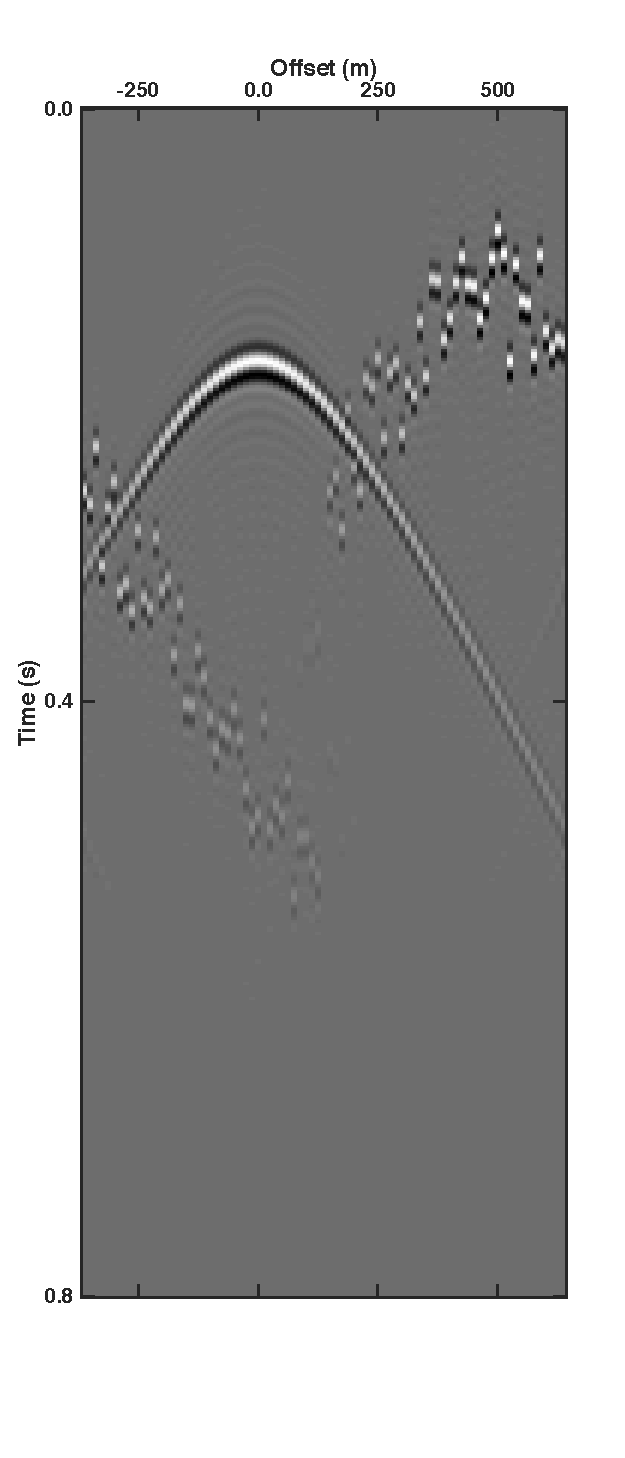
\includegraphics[width = \textwidth]{Plots/Mahdad/25iter/TimeDelay/Pseudo-DeblendedCRG_rec30}
		\caption{}
		\label{fig:Ch-Theory-PseudoCRG-IncoherentDelay}
	\end{subfigure}
	%
	\centering
	\begin{subfigure}[b]{0.3\textwidth}
	
		\centering
		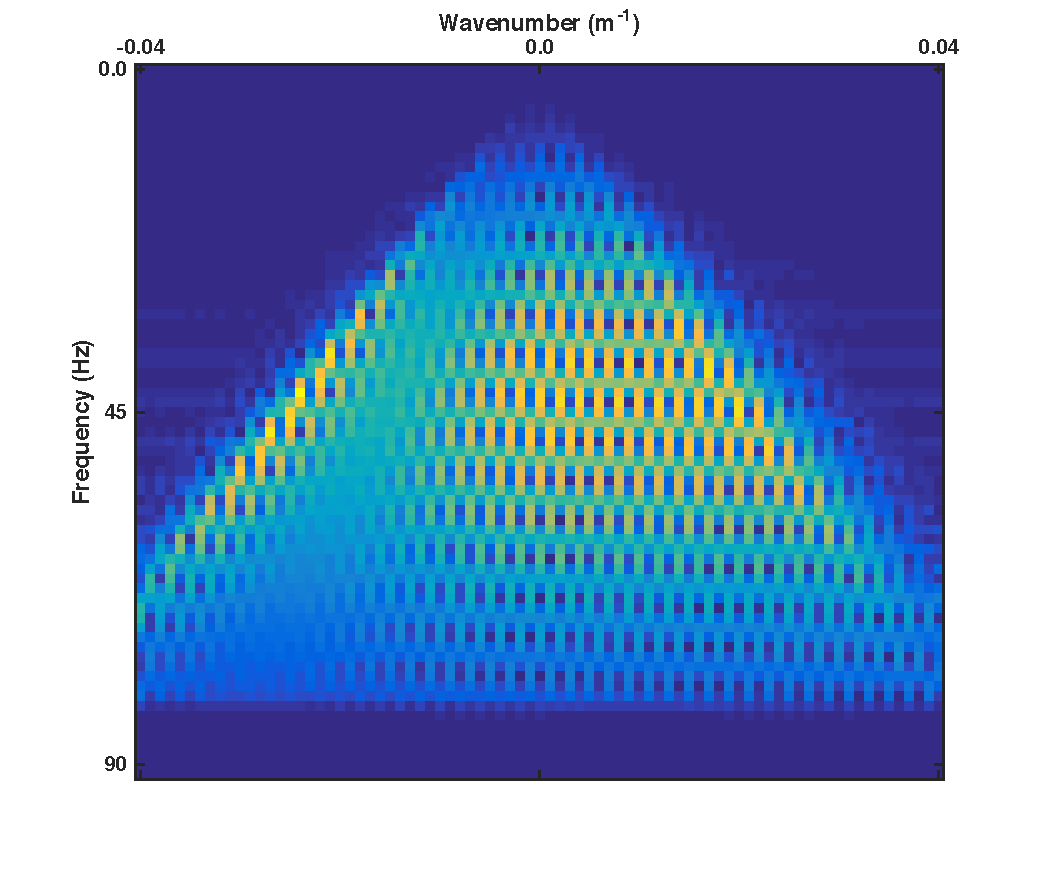
\includegraphics[width = \textwidth]{Plots/Mahdad/25iter/TimeDelay/FK-Pseudo-deblendedCRG_rec30_coh}
		\caption{}
		\label{fig:Ch-Theory-PseudoCRG-FK-CoherentDelay}
		
		\par\bigskip
		
		\centering
		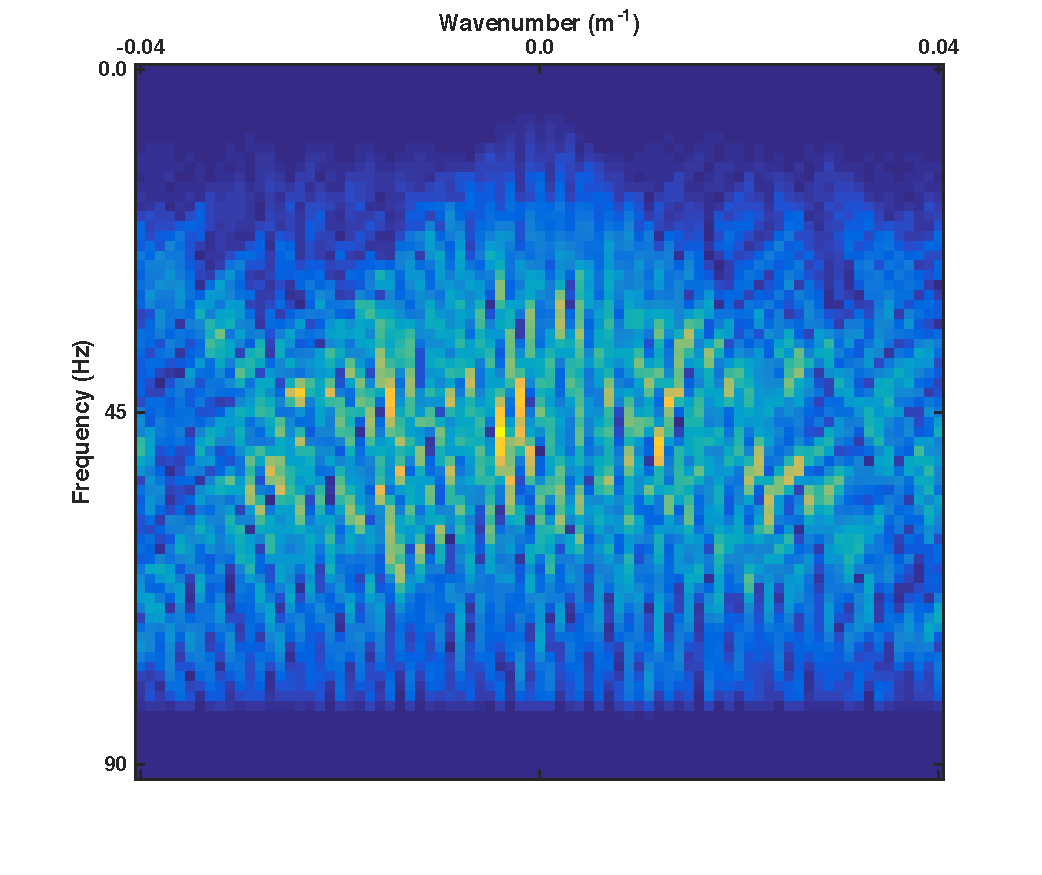
\includegraphics[width = \textwidth]{Plots/Mahdad/25iter/TimeDelay/FK-Pseudo-deblendedCRG_rec30}
		\caption{}
		\label{fig:Ch-Theory-PseudoCRG-FK-IncoherentDelay}
		
	\end{subfigure}
	
	\caption{Comparison of the pseudo-deblended receiver gather for (a) constant firing time delays of \SI{100}{\milli\second}, and (b) random firing time delays between \SI{0}{\milli\second} and \SI{100}{\milli\second}. (c) and (d) show the $f$-$k$-spectra of (a) and (b) respectively.}
	\label{fig:Ch-Theory-PseudoCRG-IncoherencyEffect}

\end{figure}

\begin{figure}
	\centering
	\includegraphics[width=\textwidth]{Plots/GGH_x_v2}
	\caption{The blending matrix, $\mathbf{\Gamma}$, is obtained by interchanging the $3^{rd}$ and $4^{th}$ row of the blending matrix in Figure \ref{fig:Ch-Theory-GGH}. In acquisition this is equivalent to moving shot 3 to experiment 2, and shot 4 to experiment 1. A random permutation of the rows of the blending matrix spreads the off-diagonal elements of the matrix product, $\mathbf{\Gamma\Gamma}^H$. The elements are not assembled on the sub-diagonals anymore.}
	\label{fig:Ch-Theory-GGHx}
\end{figure}

\begin{comment}
In order to generate incoherent source interference, $\mathbf{N}$, it is therefore favorable if the elements $a_{ik}$ of each lower or upper diagonal are out of phase. For example, considering the $n^{th}$ upper or lower diagonal of the matrix $\mathbf{\Gamma \Gamma}^H$ this observation translates to the acquisition as follows: All source pairs, which are $n$ sources apart from each other, must be fired incoherently. The incoherent firing is realized by delaying blended sources with a random time delay.
\end{comment}


\subsection*{Spatial incoherency}

Of course, the degree of incoherency of the blending noise, $\mathbf{N}$, also depends on whether the shots blended in an experiment are selected randomly, or in a spatially coherent pattern. For example, one expects the blending noise to be more incoherent if in each experiment randomly picked shots are blended, than if in each experiment adjacent shots are blended, because the interfering shots are now spread over the sub-diagonals (see Figure \ref{fig:Ch-Theory-GGHx}).

In this thesis selecting random shots for an experiment is referred to as spatial incoherency.

In practice in 2D blending shots cannot be blended in a spatially incoherent fashion, at least not in a conventional 2D marine acquisition design. In the chapter \ref{chap:MahdadMethod3d} it will be shown that blending in 3D allows to blend shots spatially incoherent within the crossline direction. 

In this chapter spatial incoherency will be illustrated with 2D synthetic data, where the acquisition design is not constraint by practicability.



\begin{comment}

In terms of the blending matrix $\mathbf{\Gamma}$ a spatially incoherent firing pattern means that the rows, i.e. the sources, are shuffled randomly. As a consequence the off-diagonal elements of the matrix product $\mathbf{\Gamma \Gamma}^H$ are reordered randomly. This shuffling process can help to further distort the phase of the interfering sources. However, if the maximum allowed time delay between blended sources is aready large the spatially incoherent blending pattern will not increase the incoherency of the interfering sources.   

In practice, the maximum allowed firing time delay is limited by the available acquisition time. The spatial distribution of blended sources is constraint by the acquisition design.
	
\end{comment}


\FloatBarrier

\section{Effect of Incoherency}

An incoherent blending pattern is crucial for good deblending performance (see section \ref{sec:BlendingMatrix}). Thus, a measure of incoherency and deblending quality will be introduced. Then, the possibilities of creating an incoherent blending pattern are presented. Finally, the effect of incoherency on the deblending quality will be shown on a synthetic data set.


\subsection*{Incoherency Measure}

\todo[inline]{Move this sentence to the introduction (literature). You might also want to mention the work of the Greek guy Apostolos.\\
In this thesis only the incoherency of the acquisition design is considered. Thus, the blending matrix, $\Gamma$, or more precisely the product $\mathbf{\Gamma \Gamma}^H$ determines the incoherency.}

A measure of incoherency will be introduced in order to analyze the importance of an incoherent blending pattern quantitatively.

In section \ref{sec:BlendingMatrix} it was shown that for an incoherent blending pattern the elements, $\mathrm{e}^{-j \omega \Delta t_{kl}}$, along a sub-diagonal of the product $\mathbf{\Gamma \Gamma}^H$ should be out of phase. Therefore, the phase variability of the sub-diagonal elements will be used to quantify incoherency.

Note that the sub-diagonal elements, $\mathrm{e}^{-j \omega \Delta t_{kl}}$, map in the complex plane on a circle with radius 1 (see Figure \ref{fig:Ch-Results-complex-circle}). 

\begin{figure}
	\centering
	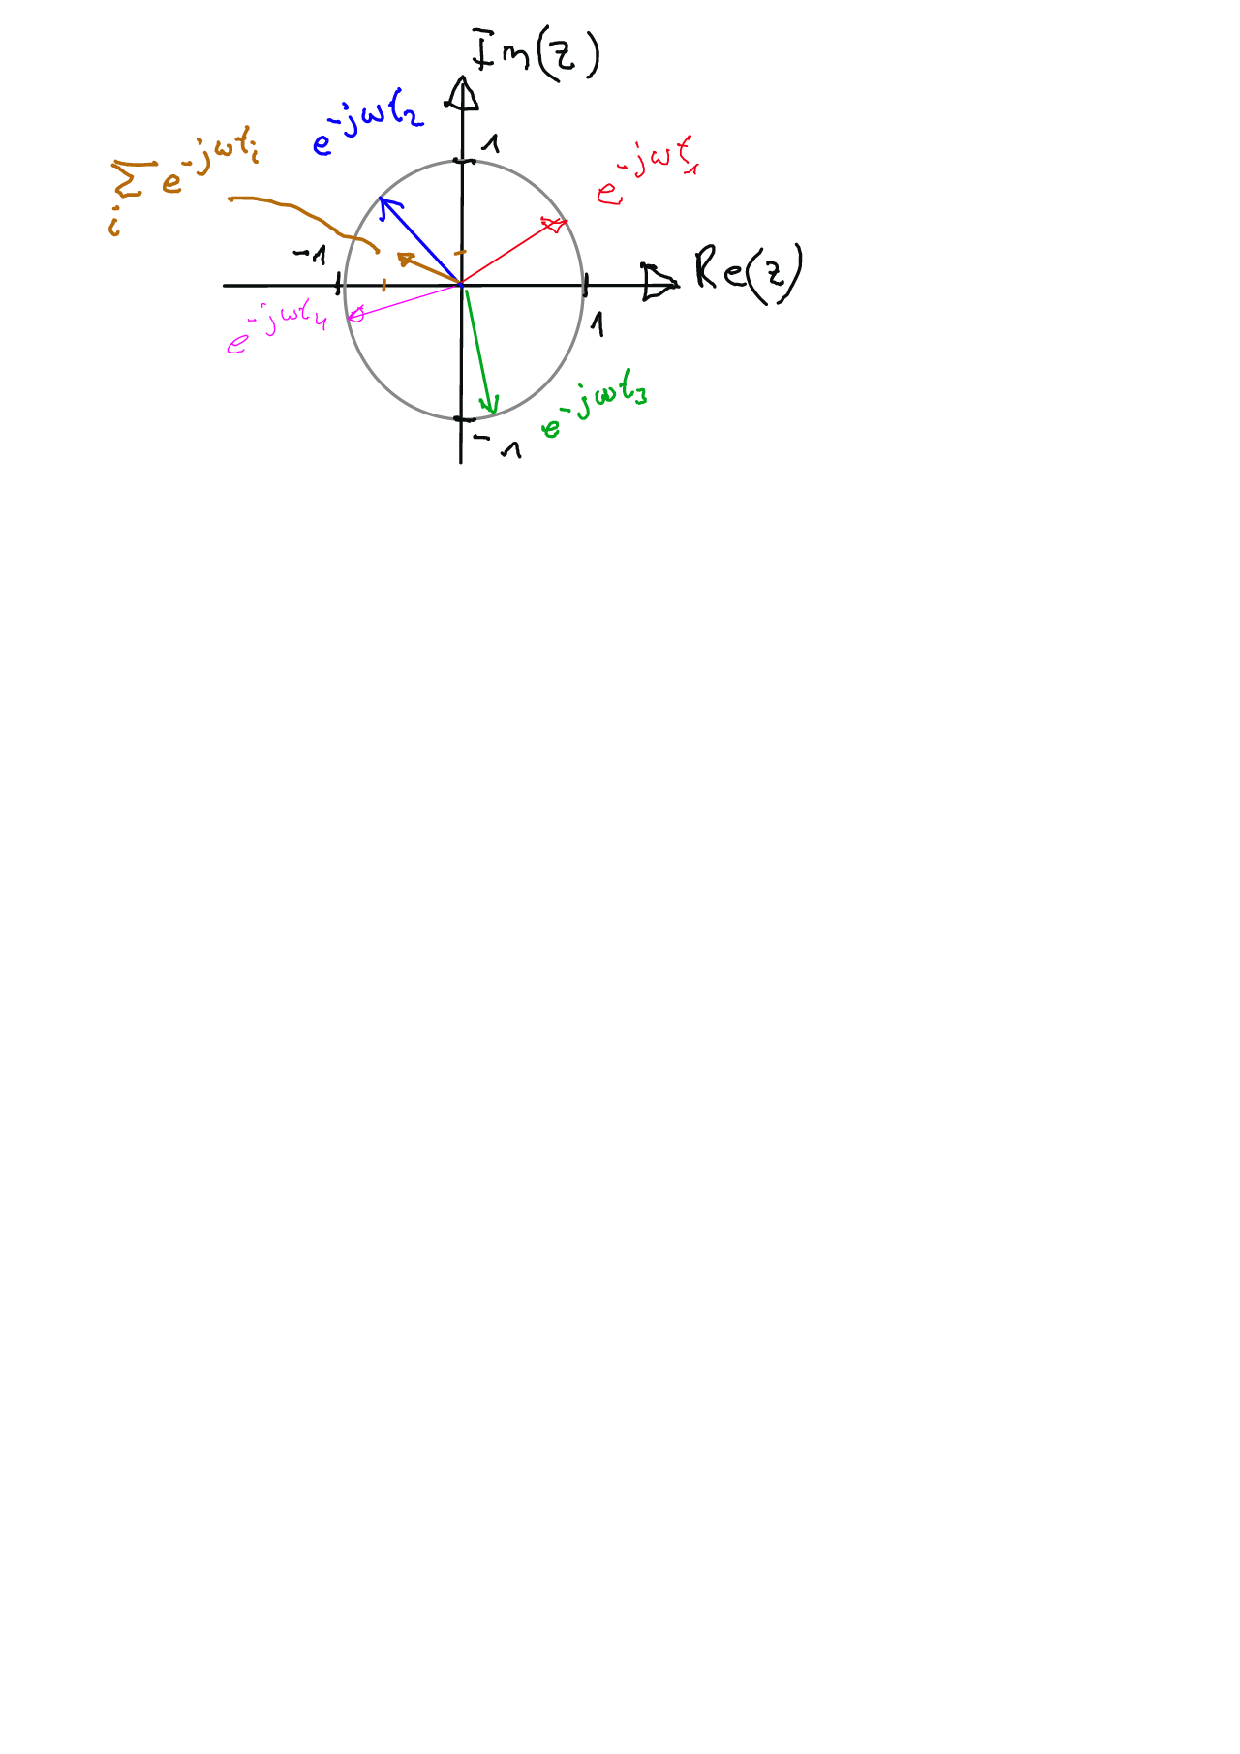
\includegraphics[width = 0.5\textwidth]{Plots/complex-circle}
	\caption{Illustration of the sub-diagonal elements in the complex number plane. The elements have unit length and variable phase. The absolute value of their sum depends on the phase coherency of the elements.}
	\label{fig:Ch-Results-complex-circle}
\end{figure}

The sum of the elements along the $k^{th}$ sub-diagonal can be constructive or destructive, depending on the phase variability. Thus, the absolute value of the sum measures the incoherency of an individual sub-diagonal. The resulting value is squared in order to put it in terms of energy;

\begin{equation}
	\left| \sum_{j-i=k} \mathbf{\Gamma \Gamma}^H_{ij} (\omega) \right|^2.
	\label{eq:Ch-Results-incoherency-diagsum}	
\end{equation} 

For example, if all elements are in phase the length of their sum is maximized. The more the elements are out of phase, i.e. the more incoherent they are, the smaller is the length of the summed elements. 

For illustration a blending matrix, $\mathbf{\Gamma}$, is generated and inserted in equation \ref{eq:Ch-Results-incoherency-diagsum}. This yields an output for each sub-diagonal, which is shown in Figure \ref{fig:Ch-Results-Diagonal-Sums}. The spike is caused by the elements on the main diagonal of $\mathbf{\Gamma \Gamma}^H$, which are all equal to 1, i.e. in phase. For a perfectly incoherent blending design the elements on a sub-diagonal cancel and the plot becomes a perfect spike. 


\begin{figure}
	\centering
	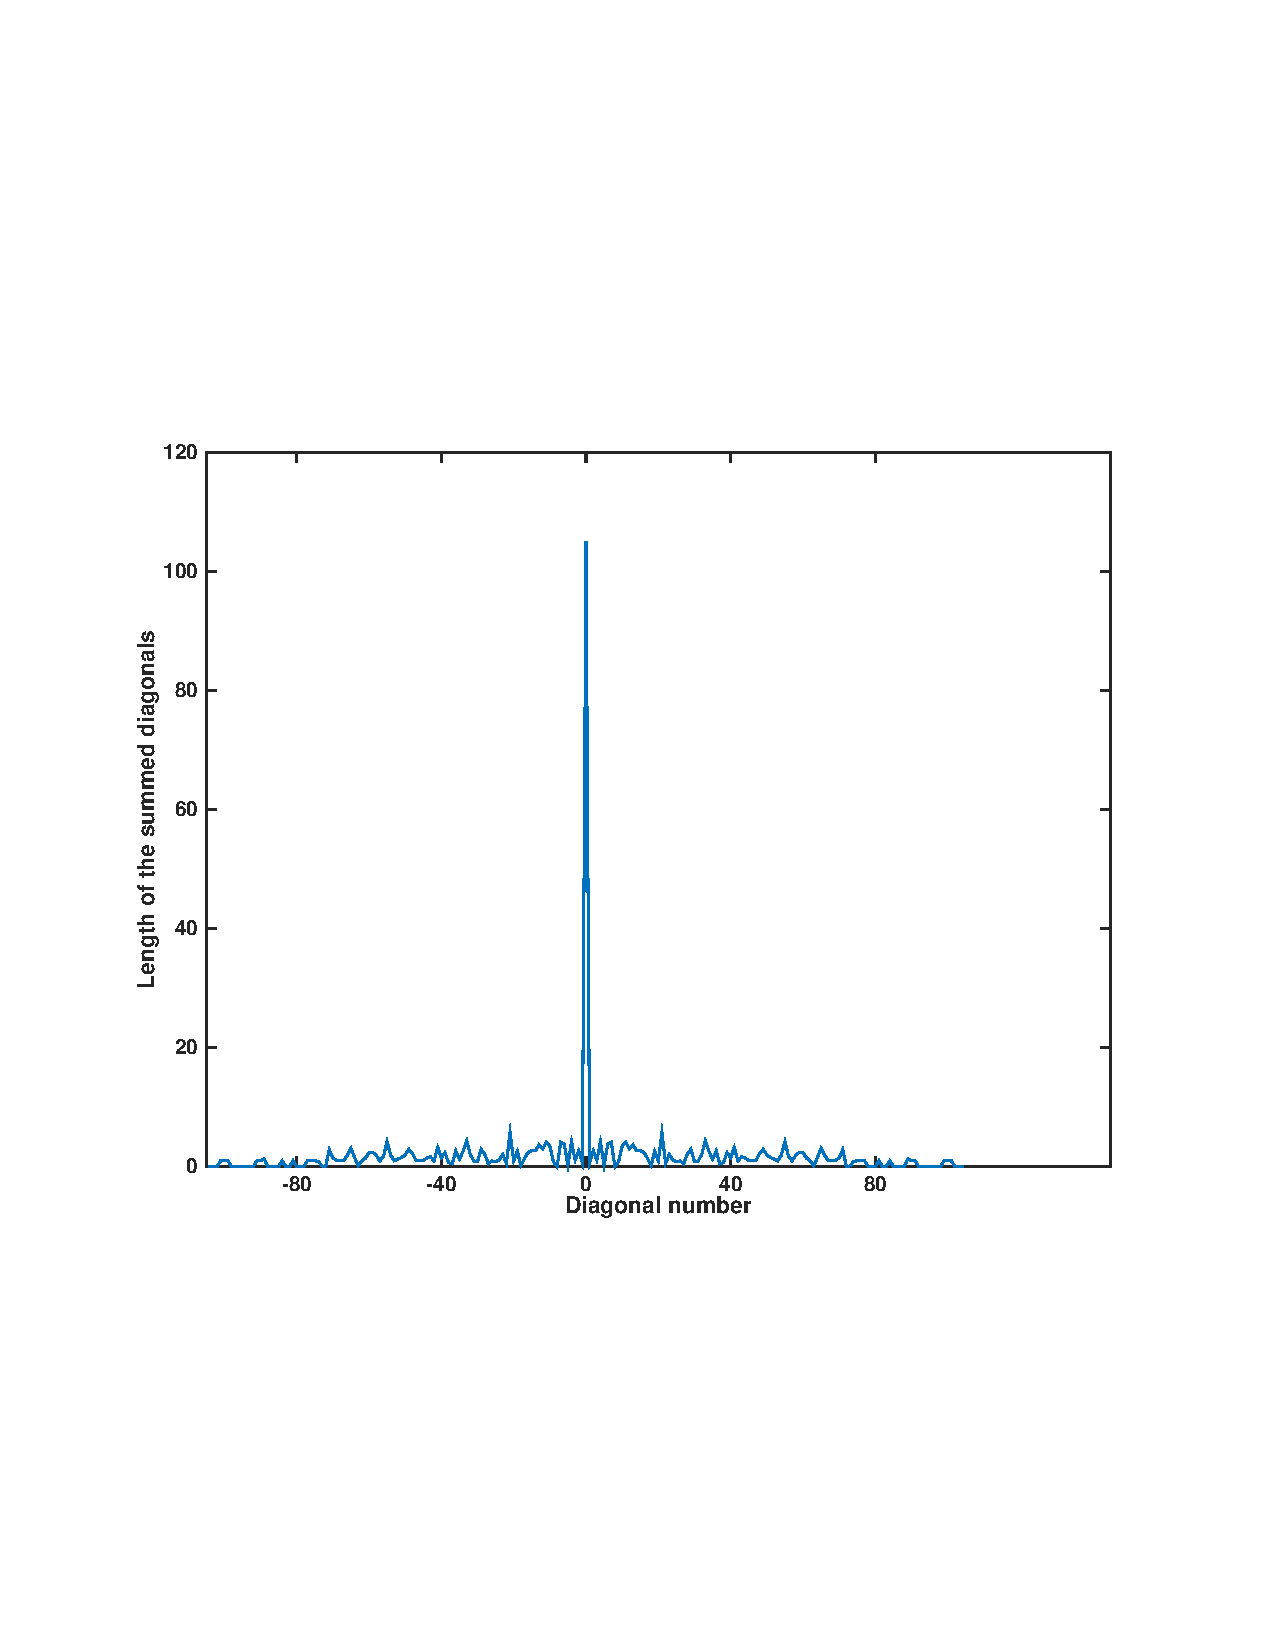
\includegraphics[width=0.6\textwidth]{Plots/diagonal-sums}
	\caption{The sub-diagonal elements, $\mathrm{e}^{-j \omega \Delta t_{kl}}$, of the product $\mathbf{\Gamma \Gamma}^H$ are summed. The length of each output is plotted. The spike is caused by the main diagonal elements of $\mathbf{\Gamma \Gamma}^H$ because they are all in phase.}
	\label{fig:Ch-Results-Diagonal-Sums}
\end{figure}

The closer Figure \ref{fig:Ch-Results-Diagonal-Sums} comes to a spike the more incoherent is the blending pattern. Thus, considering Figure \ref{fig:Ch-Results-Diagonal-Sums} the incoherency, $\mu$, is measured as the ratio between the amplitude of the spike and the sum of all amplitudes. 

In terms of the sub-diagonals of $\mathbf{\Gamma \Gamma}^H$ this is the ratio between the squared absolute value of the summed main diagonal and the sum of all squared absolute summed sub-diagonals;

\begin{equation}
	\mu(\omega) = \frac{  \left| \sum_{j-i = 0} \mathbf{\Gamma \Gamma}^H_{ij} (\omega) \right|^2    }{ \sum_{k = 1-N_s}^{N_s-1}	 \left( \left| \sum_{j-i = k} \mathbf{\Gamma \Gamma}^H_{ij} (\omega) \right|^2 \right)   }.
	\label{eq:Ch-Results-incoherency-monochromatic}
\end{equation}

Note that $N_s$ is the number of sources, i.e. the matrix $\mathbf{\Gamma \Gamma}^H$ has $N_s$ rows and columns.

Up to now, the incoherency is computed for each frequency separately. In order to account for all frequencies at once the nominator and denominator in equation \ref{eq:Ch-Results-incoherency-monochromatic} are summed over all frequency components;

\begin{equation}
	\mu = \frac{  \sum_{\omega} \left( \left| \sum_{j-i = 0} \mathbf{\Gamma \Gamma}^H_{ij} (\omega) \right|^2  \right)  }{  \sum_{\omega} \left( \sum_{k = 1-N_s}^{N_s-1}	 \left( \left| \sum_{j-i = k} \mathbf{\Gamma \Gamma}^H_{ij} (\omega) \right|^2 \right) \right)  } \;.
	\label{eq:Ch-Results-incoherency}
\end{equation}



For example, for a perfectly incoherent blending pattern only the sum along the main diagonal ($k=0$) is non zero. Thus, the nominator and the denominator in equation \ref{eq:Ch-Results-incoherency} are identical, the incoherency equals 1. 

In contrast, for a perfectly coherent blending pattern all sub-diagonal elements are in phase. Consequently, the sum along the main diagonal is of the same magnitude as the sum along the sub-diagonals. The nominator in equation \ref{eq:Ch-Results-incoherency} becomes significantly smaller than the denominator, and the incoherency is nearly 0.


\section{Results}

\section{Effect of Maximum Firing Time Delay}

\section{Results}


